\documentclass[11pt]{article}
\usepackage[margin=1in]{geometry}
\usepackage{amsmath,amssymb}
\usepackage{booktabs}
\usepackage{graphicx}
\usepackage{tikz}
\usetikzlibrary{arrows.meta,positioning,fit,backgrounds}
\usepackage[hidelinks]{hyperref}
\usepackage{natbib}

\title{Fine-to-Coarse Sequential Emotion Recognition with Hierarchical Transformer Models}
\author{TEAM MEMBERS \\ COSC 6341, Computer Science Department, TAMUCC}
\date{December 4, 2026}

\begin{document}
\maketitle

\begin{abstract}
TODO: one paragraph. State the research question (does fine-grained emotion learning on
GoEmotions improve coarse-grained sequential emotion recognition on MELD when dialogue
context is modelled by an utterance-level Transformer?), the four systems, the headline
macro-F1 numbers, and the main finding.
\end{abstract}

\section{Introduction and Motivation}
TODO: sequential emotion recognition in dialogue; why utterance-level context matters;
fine-to-coarse transfer as the central idea; the research question; contributions.

\section{Related Work}
TODO: Transformer-based emotion recognition; GoEmotions \citep{demszky2020goemotions};
conversational emotion recognition and MELD \citep{poria2019meld}; transfer learning with
RoBERTa \citep{liu2019roberta}; sequential/context modelling with Transformer encoders
\citep{vaswani2017attention}.

\section{Methodology}

\subsection{Stage I: fine-grained emotion learning}
RoBERTa-base is fine-tuned on GoEmotions over 27 fine-grained categories with the
\texttt{neutral} category excluded:
\[
x \xrightarrow{\text{RoBERTa}} h \xrightarrow{W_{27}} p(y^f \mid x),
\qquad
\mathcal{L}_f = -\sum_{k=1}^{27} y^f_k \log p(y^f_k \mid x).
\]
GoEmotions is multi-label; TODO state the reduction used (single-label examples only, or
lowest-index label) and the resulting split sizes. After training, $W_{27}$ is discarded
and the backbone parameters $\theta_G$ are retained.

\subsection{Stage II: sequential coarse emotion learning on MELD}
A dialogue is $D = (U_1, \dots, U_T)$. Each utterance is encoded by the shared
GoEmotions-trained backbone, $U_t \rightarrow h_t \in \mathbb{R}^{768}$. Turn-level
positional embeddings preserve order, $\widetilde{h}_t = h_t + p_t$, and the
utterance-level Transformer encoder contextualises the dialogue,
$(z_1, \dots, z_T) = \mathrm{UTE}(\widetilde{h}_1, \dots, \widetilde{h}_T)$, followed by
$p(y^c_t \mid D) = \mathrm{softmax}(W_7 z_t + b_7)$. The parameters
$\theta_G$, $\theta_{\mathrm{UTE}}$ and $W_7$ are all trainable in Stage~II, so Stage~II
performs continued fine-tuning rather than frozen feature extraction.

\begin{figure}[t]
\centering
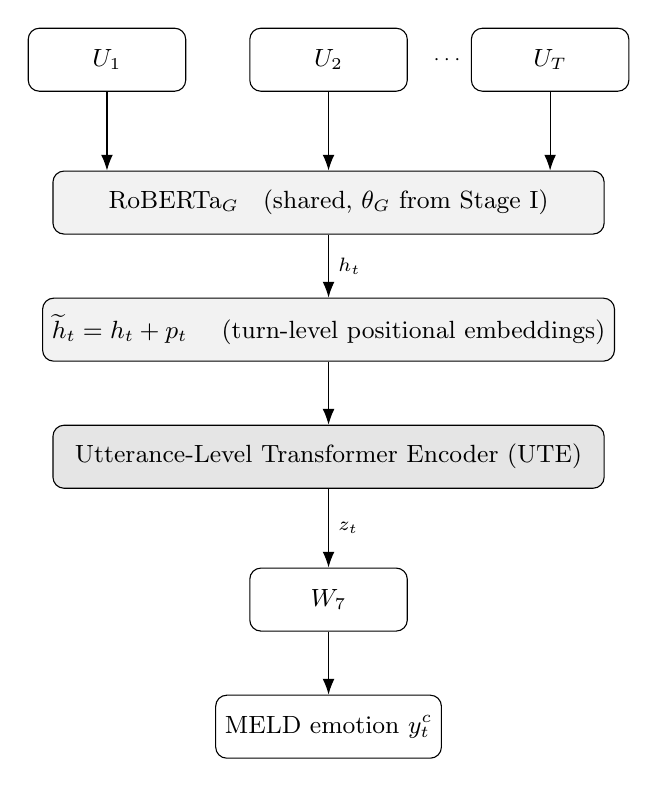
\begin{tikzpicture}[
  node distance=8mm,
  box/.style={draw, rounded corners, minimum height=8mm, minimum width=20mm, font=\small},
  small/.style={font=\scriptsize},
  arrow/.style={-{Latex[length=2mm]}}
]
\node[box] (u1) {$U_1$};
\node[box, right=of u1] (u2) {$U_2$};
\node[box, right=of u2] (ut) {$U_T$};
\node[small, right=2mm of u2] {$\cdots$};

\node[box, fill=black!5, below=10mm of u2, minimum width=70mm] (rob)
  {RoBERTa$_G$ \; (shared, $\theta_G$ from Stage I)};

\node[box, below=8mm of rob, minimum width=70mm, fill=black!5] (pos)
  {$\widetilde{h}_t = h_t + p_t$ \quad (turn-level positional embeddings)};

\node[box, below=8mm of pos, minimum width=70mm, fill=black!10] (ute)
  {Utterance-Level Transformer Encoder (UTE)};

\node[box, below=10mm of ute] (w7) {$W_7$};
\node[box, below=8mm of w7] (out) {MELD emotion $y^c_t$};

\draw[arrow] (u1) -- (u1 |- rob.north);
\draw[arrow] (u2) -- (u2 |- rob.north);
\draw[arrow] (ut) -- (ut |- rob.north);
\draw[arrow] (rob) -- node[right, small] {$h_t$} (pos);
\draw[arrow] (pos) -- (ute);
\draw[arrow] (ute) -- node[right, small] {$z_t$} (w7);
\draw[arrow] (w7) -- (out);
\end{tikzpicture}
\caption{Stage-II architecture. Systems M$_1$ and M$_2$ remove the UTE block and classify
each utterance independently; systems M$_1$ and M$_3$ start from RoBERTa-base instead of
RoBERTa$_G$.}
\label{fig:architecture}
\end{figure}

\subsection{Research extension}
TODO (only if run): the Stage-I head is kept as a frozen predictor, giving
$p^f_t \in \mathbb{R}^{27}$ per utterance; $e_t = [h_t ; p^f_t]$ is projected back to
$\mathbb{R}^{768}$ and fed to the UTE, testing whether explicit fine-grained emotion
information helps beyond transferring the backbone alone.

\section{Experimental Design}

\subsection{Datasets and preprocessing}
TODO: GoEmotions split sizes after excluding \texttt{neutral} and reducing to one label
per example; MELD 9{,}989 / 1{,}109 / 2{,}610 utterances over 1{,}039 / 114 / 280
dialogues, seven coarse categories, dialogue boundaries and utterance order preserved,
dialogues longer than $T_{\max}$ split into non-overlapping windows.

\subsection{Systems}
\begin{align*}
M_1 &: \mathrm{RoBERTa}_{base} \rightarrow \mathrm{MELD}, &
M_2 &: \mathrm{RoBERTa}_G \rightarrow \mathrm{MELD}, \\
M_3 &: \mathrm{RoBERTa}_{base} + \mathrm{UTE} \rightarrow \mathrm{MELD}, &
M_4 &: \mathrm{RoBERTa}_G + \mathrm{UTE} \rightarrow \mathrm{MELD}.
\end{align*}

\subsection{Hyperparameters and protocol}
TODO: fill from \texttt{results/<run>/metrics.json}. Learning rates, batch size, epochs,
maximum sequence length, $T_{\max}$, UTE depth / heads / feed-forward size, dropout,
optimiser, warmup, gradient clipping, seed. Model selection is by dev macro-F1; the test
set is used once, for the final numbers only.

\subsection{Evaluation metrics}
Accuracy, macro-F1 and weighted-F1, with per-class precision, recall and F1. MELD is
class-imbalanced, so macro-F1 is the primary metric.

\section{Results and Analysis}
% Placeholder -- regenerated by: python scripts/build_results_table.py
\begin{table}[t]
\centering
\caption{MELD test results for the four required systems (\%).}
\label{tab:main}
\begin{tabular}{lccccc}
\toprule
Model & GoEmotions & UTE & Accuracy & Macro-F1 & Weighted-F1 \\
\midrule
$M_1$ & No & No & -- & -- & -- \\
$M_2$ & Yes & No & -- & -- & -- \\
$M_3$ & No & Yes & -- & -- & -- \\
$M_4$ & Yes & Yes & -- & -- & -- \\
\bottomrule
\end{tabular}
\end{table}


TODO: interpret the three comparisons --- $M_1$ vs $M_2$ (fine-grained transfer),
$M_1$ vs $M_3$ (sequential context), $M_3$ vs $M_4$ (transfer on top of context) ---
and the per-class table. Which emotion categories gain from transfer, which gain from
context, and where the models still fail.

\section{Error Analysis}
TODO: representative correct and incorrect predictions from
\texttt{docs/tables/error\_analysis.json}. Ambiguous utterances; the minority classes
(\texttt{disgust}, \texttt{fear}); dialogue dependencies; cases where conversational
context changes the emotion interpretation; the dominant confusion pairs.

\section{Conclusion}
TODO: major findings, limitations (text-only, window truncation, single seed unless
repeated), future work. Clearly separate implemented work, experimental findings, and
proposed future work.

\bibliographystyle{plainnat}
\bibliography{report}

\end{document}
